% Repo as Root Disk
%
% IEEEtran's journal layout, the format the author prefers for this paper. The
% venue's own template is the Computer Society one (the compsoc option), and its
% 12-page limit is counted in that layout, so a page count here is not the
% venue's page count.
%
% Build: sh build.sh (generates results and cross-references, then LaTeX)

\documentclass[journal,10pt]{IEEEtran}

% Accented names in the bibliography compose as an accent over a letter
% without this, which prints correctly but extracts as mojibake, breaking
% copy-paste and indexing.
\usepackage{cmap}
\usepackage[T1]{fontenc}
\usepackage{amsmath}
\usepackage{booktabs}
% Paragraph columns set ragged right: justified narrow cells stretch the
% spaces between words into gaps.
\usepackage{array}
\newcolumntype{P}[1]{>{\raggedright\arraybackslash}p{#1}}
\usepackage{algorithm}
\usepackage{algpseudocode}
\usepackage{url}
\usepackage{cite}
\usepackage{tikz}
\usetikzlibrary{positioning,arrows.meta,fit,backgrounds,calc}
\usepackage[hidelinks]{hyperref}
\hypersetup{pdftitle={Repo as Root Disk: A Code Hosting Service as the Backing Store for Browser-Native Virtual Machines}, pdfauthor={Prasad Patil}}

% Pointers into the supplement are generated from its label file by xref.mjs,
% never typed (AGENTS.md 3.3): \Sref{label} prints the supplement's own number.
% An unknown label prints ?? and warns, as \ref does.
\makeatletter
\newcommand{\Sref}[1]{\@ifundefined{xr@S@#1}{\textbf{??}\@latex@warning{Reference `#1' in the supplement undefined}}{\@nameuse{xr@S@#1}}}
\makeatother
\InputIfFileExists{xref-supplement.tex}{}{}

% Every experimental number is generated from traces/ by results.mjs, never
% typed (AGENTS.md 3.1): \R{key} prints it. An unknown key prints ?? and warns.
\makeatletter
\newcommand{\R}[1]{\@ifundefined{r@#1}{\textbf{??}\@latex@warning{Result `#1' undefined}}{\@nameuse{r@#1}}}
\makeatother
\InputIfFileExists{generated/results.tex}{}{}
% Generated table and figure bodies. \@@input is TeX's own input, which,
% unlike LaTeX's \input, is expandable and so may sit inside a tabular.
\makeatletter
\newcommand{\gen}[1]{\@@input generated/#1 }
\makeatother

% Diagram palette. Gray carries structure, one accent marks the path the
% contribution is about, so a reader can find it without a legend.
\definecolor{ink}{HTML}{1A1A1A}
\definecolor{rule}{HTML}{9A9A9A}
\definecolor{soft}{HTML}{EFEFEF}
\definecolor{accent}{HTML}{1F5C4D}
\definecolor{accentsoft}{HTML}{DCEAE5}

% A column heading on two lines, which fits a narrow column without
% shrinking the table's type.
\newcommand{\hd}[1]{\begin{tabular}[b]{@{}c@{}}#1\end{tabular}}

\begin{document}
% Must be the first citation: IEEEtran.bst applies these controls
% in citation order, so later is too late.
\bstctlcite{IEEEexample:BSTcontrol}

\title{Repo as Root Disk: A Code Hosting Service as the\\
Backing Store for Browser-Native Virtual Machines}

\author{
\IEEEauthorblockN{
$^1$,$^2$Prasad Patil
}\\
\IEEEauthorblockA{
$^1$Department of Computer Science and Engineering\\
Indian Institute of Information Technology Nagpur, India $-$ 441108\\
dtei24cse008@iiitn.ac.in
} \\
\IEEEauthorblockA{
$^2$Tata Consultancy Services, Nagpur, India\\
p.ppatil@tcs.com
}}

\IEEEtitleabstractindextext{%
\begin{abstract}
Virtual machines now run inside a web browser, but their disks
are read only: a user's work stays in one browser and is lost when its data is
cleared. Teaching, demonstrations and reproducible
research need machines that survive and move between devices without a server.
We know of no system that writes such a disk back to storage its user owns. We
keep the disk in a source-code hosting service, saving each batch of
changed blocks as a new version. We built a working system, ran it on two
hosting services, raced concurrent writers on four, and compared it over a thousand simulated saves with two other
designs and a backup tool. Restoring a machine reads only the blocks it
currently holds, so its cost depends on the disk, not the number of saves. A design that replays
its history grew with every save, and so did the backup tool until its index was
rebuilt. In a browser, a round trip from a write to a rebuilt machine took
about \R{br.roundTrip} seconds. Installed software survived a rebuild. The main limit is the
service: it caps requests, and one of the four can lose a save when two devices
write together.
\end{abstract}

\begin{IEEEkeywords}
Storage services, service measurement, browser-based virtualization,
content-addressable storage, rate limiting, service portability, WebAssembly.
\end{IEEEkeywords}}

\maketitle
\IEEEdisplaynontitleabstractindextext
\IEEEpeerreviewmaketitle

\section{Introduction}
\label{sec:intro}

A browser tab can now boot Linux. Emulators such as v86 and virtualization
engines such as CheerpX run unmodified x86 binaries client side, with no
server, and projects built on them ship Linux environments as static web pages.

All of them share a limitation that is easy to miss because it is uniform:
\emph{the disk is read only}. A pre-built image is streamed over HTTP, writes
land in browser-local storage, and an overlay merges the two; no block is ever
written back, so machine state is trapped. It cannot be moved to another device,
shared, reviewed, archived or cited, and clearing site data destroys it.

This paper closes that loop, which to our knowledge no prior system does. We
commit the guest's changed blocks into a code hosting service, or \emph{forge},
as ordinary git objects. A machine's state then becomes a commit and its
history a git history. Fork, checkout and bisect apply to a running environment,
and any device can rebuild the machine from a branch name alone.

The mechanism is small. Building it required characterizing a forge as a block
storage tier, which we found no prior measurement of. That characterization is
the larger part of our contribution, and several of its results are negative.
Almost none of the behavior we report comes from the emulator. It comes from a
storage tier that meters requests rather than bytes, prices a small write and a
large one alike, and touches one object at a time. Such interfaces are common
and rarely designed as storage, so the rules transfer
(Section~\ref{sec:rules}), and the same engine also drives a Linux kernel block
device.

\paragraph{Contributions}
\begin{enumerate}\itemsep2pt
\item A write-back block device for browser-native virtual machines that needs
no change to the emulator, and a sync protocol that turns a machine's state into
a commit (Section~\ref{sec:design}). Restore reads only the \emph{live set}, the
chunks the disk currently needs, so its cost grows with what the disk holds and
never with the number of syncs. It held at \R{scale.ours.req} requests from sync \R{scale.half} to sync \R{scale.syncs}, where
a replaying design reached \R{scale.delta.req1000} (Section~\ref{sec:scaling}). The deployment operates no server.
\item A committed device that carries a general-purpose Linux userland rather
than a scratch partition. Alpine installs packages onto it offline, and they
reappear on a machine rebuilt from the repository (Section~\ref{sec:alpine}).
The image's kernel also boots the rebuilt device as its root filesystem, with
the distribution's own shell as process~1; only the kernel stays outside it.
\item Evidence that the design is not tied to the browser. The device contract
has five operations and names no emulator, and a third implementation serves a
Linux kernel over the Network Block Device (NBD) protocol with the same engine.
A Linux \R{kern.release} kernel formatted, wrote and remounted a machine rebuilt from the
repository through it. On both guests, a sync that skipped the flush committed a
disk without the file just written, so the flush requirement is not an emulator
quirk (Section~\ref{sec:kernel}).
\item A measurement study of a forge used as block storage
(Sections~\ref{sec:tier} to~\ref{sec:contention}). No write was refused below
\R{env.passRate} a minute, against a documented limit of 80~\cite{ghratelimits}. Three negative results
constrain the design. Within a disk, deduplication saves only free space, a
format's structure and copies: \R{occ.fullDisk} times on a disk \R{occ.fullUse} full, and nothing among a distribution's files.
Compaction is bound by the rate a client can rely on, not by bandwidth. The
object interface the design needs is the most expensive in requests of the
three services' interfaces, measured on two and documented on the third.
\end{enumerate}

\paragraph{Scope} We claim no performance result for Linux on NBD, no
benchmark of any object store, and no concurrency safety beyond what each
host's atomic primitive gives. That safety is per commit, and a filesystem
needs one active writer per branch. The design suits machines a person changes
in bursts, for teaching, demonstration or a reproducible artefact, not a
database: a 1\,GB machine takes \R{gb.github.commitMinutes} minutes to commit. Section~\ref{sec:related} reviews related work,
Section~\ref{sec:design} gives the design and its implementation,
Section~\ref{sec:eval} the measurements and Section~\ref{sec:limits} the
limitations. The implementation, the harnesses and the traces are
archived~\cite{artifact}.

\section{Background and Related Work}
\label{sec:related}

Four families of system overlap with ours, and none occupies the same point.
Table~\ref{tab:related} summarizes them.

\begin{table*}[t]
\caption{Related systems, representative ones for each family; Section~\ref{sec:related}
names more. \textsuperscript{*}Binder versions the recipe
rather than the state, and sessions are ephemeral. Only this work combines client-side execution with versioned, cross-device state
at block granularity and no infrastructure of its own. ``Operator cost'' is
what the deployment runs, not what the backing service charges.}
\small
\centering
\begin{tabular}{@{}llccclc@{}}
\toprule
& & client-side & state across & versioned & & operator \\
family & representative systems & execution & devices & history & granularity & cost \\
\midrule
browser machines
  & v86~\cite{v86} & $\bullet$ & & & none & zero \\
  & JSLinux~\cite{jslinux} with vfsync~\cite{vfsync} & $\bullet$ & $\bullet$ & & file & server \\
  & WebVM / CheerpX~\cite{webvm} & $\bullet$ & & & block & zero \\
  & container2wasm~\cite{c2w} & $\bullet$ & & & none & zero \\
  & WebContainers~\cite{webcontainers} & $\bullet$ & & & file & vendor \\
\addlinespace
hosted environments
  & OnWorks~\cite{onworks} & & $\bullet$ & & image & server \\
  & Codespaces~\cite{codespaces} & & $\bullet$ & & file & paid \\
  & Binder / repo2docker~\cite{binder,repo2docker} & & & $\bullet$\rlap{\,\textsuperscript{*}} & image & BinderHub \\
  & Code Ocean~\cite{codeocean}, Whole Tale~\cite{wholetale} & & $\bullet$ & $\bullet$ & image & platform \\
\addlinespace
versioned storage
  & Venti~\cite{venti} & & $\bullet$ & $\bullet$ & block & server \\
  & bup~\cite{bup}, git-annex~\cite{gitannex}, LFS~\cite{gitlfs} & & $\bullet$ & $\bullet$ & chunk/file & none \\
  & restic~\cite{restic}, Borg~\cite{borg}, casync~\cite{casync} & & $\bullet$ & $\bullet$ & chunk & none \\
  & gitfs~\cite{gitfs}, RepoFS~\cite{repofs} & & $\bullet$ & $\bullet$ & file & none \\
\addlinespace
\textbf{this work} & & $\bullet$ & $\bullet$ & $\bullet$ & block & zero \\
\bottomrule
\end{tabular}

\label{tab:related}
\end{table*}

\paragraph{Browser-native machines}
JSLinux~\cite{jslinux} first showed a browser-hosted x86 machine.
v86~\cite{v86} translates x86 to WebAssembly at runtime and boots Alpine,
Buildroot and Arch from static files. CheerpX, used by WebVM~\cite{webvm},
executes unmodified Debian binaries against a virtual block-based filesystem.
container2wasm~\cite{c2w} converts container images to WebAssembly bundles, and
WebContainers~\cite{webcontainers} runs Node.js compiled to WebAssembly. In
every case the disk is fetched read only; CheerpX documents an overlay that
keeps changes in IndexedDB, with no path back to the image~\cite{cheerpx}. The one write path
off the client, JSLinux's vfsync, syncs a directory mounted over the 9P
protocol~\cite{jslinuxtech} to the vfsync service~\cite{vfsync}; the disk stays read only.
Browsix~\cite{browsix} and Doppio~\cite{doppio} give browser programs Unix
services instead of a machine, and Doppio's file system reaches cloud storage a
file at a time. We write the disk back to storage its user owns.

\paragraph{Hosted environments}
The alternative is to move execution to a server. OnWorks~\cite{onworks} gets
ownership right and execution wrong: workstations run on its servers, and the
whole system saves to the user's Google Drive as one image file.
Codespaces~\cite{codespaces} persists workspaces at file granularity on paid
infrastructure. Binder~\cite{binder} with
repo2docker~\cite{repo2docker} is closest to our reproducibility motivation but
versions the \emph{recipe} rather than the state; Code Ocean~\cite{codeocean}
and Whole Tale~\cite{wholetale} package code, data and environment for
reproduction on managed platforms. All three ship container images;
Nix~\cite{nix} reproduces an environment from a description. We keep execution
on the client and version the machine's state, not its recipe.

\paragraph{Versioned and content-addressed storage}
Venti~\cite{venti} established the model we rely on: blocks addressed by the
hash of their contents, written once, with duplicate writes coalescing.
IPFS~\cite{ipfs} later combined content addressing with versioning at internet
scale. bup~\cite{bup}, git-annex~\cite{gitannex} and Git LFS~\cite{gitlfs} keep
large or backed-up data beside a repository. restic~\cite{restic},
Borg~\cite{borg} and casync~\cite{casync} apply content-defined chunking to
backups and image distribution. Duplicacy~\cite{duplicacy} keeps a
content-addressed store consistent on a passive object store, with lock-free
deduplication and no coordinating server, and Boafft~\cite{boafft} scales
deduplication across a cluster. gitfs~\cite{gitfs} and RepoFS~\cite{repofs}
expose git repositories as filesystems. Irmin~\cite{irmin} keeps an
application's data in Git's on-disk format, and Dolt~\cite{dolt} gives a SQL
database Git's branches on a storage engine of its own. For virtual machine images,
Mirage~\cite{mirage} keeps a manifest from file names to content in a store many
images share, and OSTree~\cite{ostree} versions operating-system trees in a
git-like object store, both a file at a time. Jin and Miller~\cite{jinmiller}
deduplicated whole disk images and found fixed-size chunks nearly as good as
variable-size ones, and zero-filled blocks alone worth finding. s3backer~\cite{s3backer}
keeps a block device on S3, one object per block, and stores no zero block.

Two assumptions run through all of them: the client is an operating-system
process with filesystem access and an unmetered connection, and the store is
passive and holds bytes. Neither holds here. Our client is a browser tab with no
filesystem, and our store is an interactive service that meters writes, budgets
requests rather than bytes, and offers a different write application
programming interface (API) on each provider.
Cumulus~\cite{cumulus} is the exception on cost: it backs up to a store with
only put, get, list and delete, and groups data into segments to trade the
store's per-request charges against its per-byte ones. BlueSky~\cite{bluesky}
serves a file system from such a store through a log of segments. Both still
price requests in money, not against a ceiling, from an operating-system
process. Duplicacy's lock-free argument is the closest precedent for our compare-and-swap
on a reference, and the difference is instructive: it can assume a store
accepting any number of puts, where our write rate binds the whole design.
Delta Lake~\cite{deltalake} commits a table by creating its log's next record
with an atomic put-if-absent; on S3, which had none, it ran a coordination
service of its own.

\paragraph{Storage from static hosting}
sql.js-httpvfs~\cite{httpvfs} serves a read-only SQLite database from static
hosting by range requests, the technique under streamed disk images too, and
the Origin Private File System~\cite{opfs} persists locally, to one device. A
forge can also be the storage tier for a static application outright:
MindSpark~\cite{mindspark} keeps a user's documents in a repository their own
account owns, with no backend, across GitHub, Gitea and Forgejo. That is our
substrate and no-server pattern at a coarser granularity, and the closest
existing work to ours. What it lacks is the block device: a file rewritten in
full has no partial state to reconcile, and every constraint here comes from
that gap.

\paragraph{Moving and restoring machine state}
Internet Suspend/Resume~\cite{isr} layered virtual machines on a distributed
file system so a suspended machine resumes on another computer. The
Collective~\cite{collective} keeps versioned machine images in a repository
that clients cache and write back to, and Foundation~\cite{foundation} archives
every nightly state of a user's machine in a content-addressed store. Each runs
its own store and client software; none writes back from a browser.
Firecracker~\cite{firecracker} serializes a running microVM and its resources so
a later process resumes it rather than boots it~\cite{fcsnap}. That is our restore problem at a
scale we do not approach, on a store tuned for latency where ours meters requests.

\paragraph{The gap}
Browser disks do not write back. Hosted environments write back but execute
elsewhere and cost money to run. Versioned stores do neither from a browser.
Static-host storage writes back whole documents, not blocks. We combine client-side execution with
versioned, cross-device, user-owned state, and the price of that combination is
what the rest of this paper measures.

\section{Design}
\label{sec:design}

Fig.~\ref{fig:stack} shows the three parts: a device layer that captures the
guest's writes, a commit shape that turns each epoch into git objects, and a
sync protocol between them. Several choices below follow from measurement
rather than from documentation, and Section~\ref{sec:impl} gives the
implementation.

\begin{figure}[t]
\centering

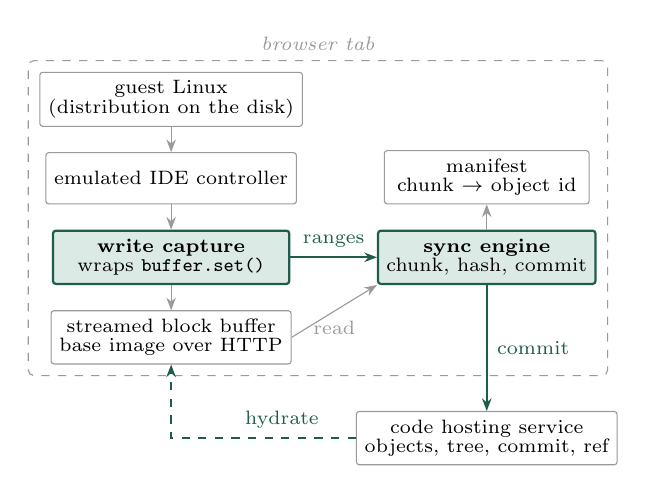
\begin{tikzpicture}[
  font=\scriptsize,
  box/.style={
    draw=rule,
    fill=white,
    rounded corners=1pt,
    align=center,
    inner sep=3pt,
    minimum height=6.5mm
  },
  hot/.style={
    box,
    draw=accent,
    fill=accentsoft,
    thick
  },
  lbl/.style={
    font=\scriptsize\itshape,
    text=rule
  },
  flow/.style={
    -{Stealth[length=1.6mm]},
    draw=rule
  },
  keyflow/.style={
    -{Stealth[length=1.6mm]},
    draw=accent,
    thick
  }
]

% --------------------------------------------------------------------------
% Browser side
% --------------------------------------------------------------------------

\node[box, minimum width=30mm] (guest)
  {guest Linux\\[-1pt]\scriptsize(distribution on the disk)};

\node[box, minimum width=30mm, below=3.2mm of guest] (ide)
  {emulated IDE controller};

\node[hot, minimum width=30mm, below=3.2mm of ide] (wrap)
  {\textbf{write capture}\\[-1pt]\scriptsize wraps \texttt{buffer.set()}};

\node[box, minimum width=30mm, below=3.2mm of wrap] (buf)
  {streamed block buffer\\[-1pt]\scriptsize base image over HTTP};

\node[hot, minimum width=26mm, right=11mm of wrap] (engine)
  {\textbf{sync engine}\\[-1pt]\scriptsize chunk, hash, commit};

\node[box, minimum width=26mm, above=3.2mm of engine] (man)
  {manifest\\[-1pt]\scriptsize chunk $\rightarrow$ object id};

% --------------------------------------------------------------------------
% Code hosting service -- deliberately OUTSIDE the browser-tab boundary
% --------------------------------------------------------------------------

\node[box, minimum width=31mm, below=16mm of engine] (host)
  {code hosting service\\[-1pt]\scriptsize objects, tree, commit, ref};

% --------------------------------------------------------------------------
% Browser-tab boundary
% --------------------------------------------------------------------------

\begin{scope}[on background layer]
  \node[
    draw=rule,
    dashed,
    rounded corners=2pt,
    inner sep=4pt,
    fit=(guest)(buf)(man)(engine),
    label={[lbl]above:browser tab}
  ] (tab) {};
\end{scope}

% --------------------------------------------------------------------------
% Internal browser-side flow
% --------------------------------------------------------------------------

\draw[flow] (guest) -- (ide);
\draw[flow] (ide) -- (wrap);
\draw[flow] (wrap) -- (buf);

% Block ranges sent from capture to sync engine
\draw[keyflow]
  (wrap.east) -- node[above, font=\scriptsize, text=accent] {ranges} (engine.west);

% Engine reads chunk contents back through the buffer
\draw[flow]
  (buf.east) -- node[below, font=\scriptsize, text=rule] {read} (engine.south west);

% Engine produces/uses the manifest
\draw[flow]
  (engine) -- (man);

% --------------------------------------------------------------------------
% Browser <-> hosting service
% --------------------------------------------------------------------------

% Commit path: directly downward from sync engine
\draw[keyflow]
  (engine.south)
  -- node[right, font=\scriptsize, text=accent] {commit}
  (host.north);


% Hydration path: code hosting service -> streamed block buffer
\draw[keyflow, dashed]
  (host.west)
  -- ++(0,0)
  -| node[above, font=\scriptsize, text=accent, pos=0.2] {hydrate}
  (buf.south);





\end{tikzpicture}

\caption{The device stack. Capture wraps one method on the emulator's block
buffer and records byte ranges, not payloads. The engine reads chunk contents
back through the same buffer when it needs them, so the emulator merges the base
image and everything written over it, with no shadow copy. Hydration is the
reverse path, and it must run before capture is armed or the restored disk is
recorded as the guest's own work.}
\label{fig:stack}

\end{figure}



\subsection{Device layers}

The guest sees one block device over a read-only base image. Existing systems
stream that image over HTTP with range requests. Every disk our application
offers has a blank base, which the page builds as zeros without a download. We add two
elements: a \emph{capture wrapper} around the device's write path, and a
\emph{sync engine} that turns what it records into objects in the service.

The \emph{manifest}, a file committed with every sync, records two things per
chunk. One is the object id, which is the address and, because we store git
objects, a SHA-1 hash. The other is a SHA-256 digest of the chunk as stored,
which restore and hydration check before anything reaches the disk.
Section~\ref{sec:limits} says what that does and does not buy.

The contract between the engine and the device is deliberately narrow: a size,
a flush, a way to close and read back the current epoch of writes, a chunk read,
and an unrecorded write used for putting a machine back. Five operations, none of
which mentions an emulator. We implement it three times, in memory for the tests,
over v86's buffer for the browser, and over NBD for a Linux kernel
(Section~\ref{sec:kernel}).

The wrapper records byte ranges, not payloads. Shadowing modified blocks in a
local store, as existing browser machines do, would put a second disk in the
tab, while the emulator already merges the base with everything written over
it. The range log for a full disk is a few kilobytes.

The two directions cost differently, and the asymmetry drives the design. Reads
of a base image, where there is one to read, are ordinary static hosting:
cacheable, ranged and outside the API. Writes draw on a small per-minute allowance, so the boot path stays off
the API and the allowance goes to commits. We had expected reads of
\emph{committed} objects to be as cheap, from the delivery host that fronts raw
repository files. Section~\ref{sec:tier} reports why they are not for a private
repository, so restore reads come from the API and count against the same budget
as writes.

\begin{figure}[t]
\centering
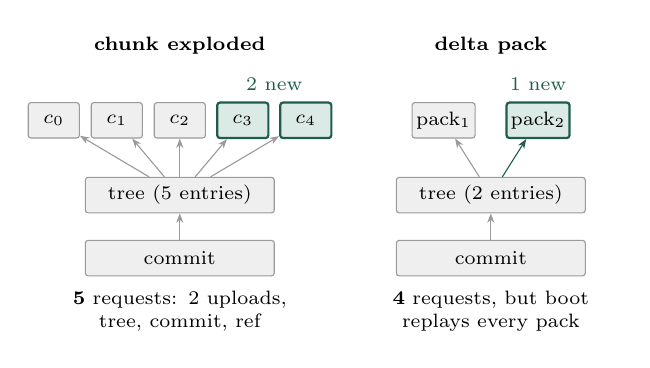
\begin{tikzpicture}[
  font=\scriptsize,
  obj/.style={draw=rule, fill=soft, rounded corners=1pt, minimum width=6.5mm,
              minimum height=4.5mm, inner sep=1pt, font=\scriptsize},
  new/.style={obj, draw=accent, fill=accentsoft, thick},
  hdr/.style={font=\scriptsize\bfseries},
  ref/.style={-{Stealth[length=1.2mm]}, draw=rule},
  newref/.style={-{Stealth[length=1.2mm]}, draw=accent},
  note/.style={font=\scriptsize, anchor=north, align=center, text width=31mm}
]

% --- chunk exploded -------------------------------------------------------
\node[hdr] (t1) at (1.0,0.15) {chunk exploded};
\node[obj] (a1) at (-0.6,-0.80) {$c_0$};
\node[obj] (a2) at (0.2,-0.80)  {$c_1$};
\node[obj] (a3) at (1.0,-0.80)  {$c_2$};
\node[new] (a4) at (1.8,-0.80)  {$c_3$};
\node[new] (a5) at (2.6,-0.80)  {$c_4$};
\node[font=\scriptsize, text=accent, anchor=south] at (2.2,-0.54) {2 new};
\node[obj, minimum width=24mm] (tree1) at (1.0,-1.75) {tree (5 entries)};
\node[obj, minimum width=24mm] (cm1) at (1.0,-2.55) {commit};
\foreach \n in {a1,a2,a3,a4,a5} { \draw[ref] (tree1) -- (\n); }
\draw[ref] (cm1) -- (tree1);
\node[note] at (1.0,-2.85) {\textbf{5} requests: 2 uploads, tree, commit, ref};

% --- delta pack -----------------------------------------------------------
\begin{scope}[xshift=4.35cm]
\node[hdr] (t2) at (0.6,0.15) {delta pack};
\node[obj, minimum width=8mm] (p1) at (0.0,-0.80) {pack$_1$};
\node[new, minimum width=8mm] (p2) at (1.2,-0.80) {pack$_2$};
\node[font=\scriptsize, text=accent, anchor=south] at (1.2,-0.54) {1 new};
\node[obj, minimum width=24mm] (tree2) at (0.6,-1.75) {tree (2 entries)};
\node[obj, minimum width=24mm] (cm2) at (0.6,-2.55) {commit};
\draw[ref] (tree2) -- (p1);
\draw[newref] (tree2) -- (p2);
\draw[ref] (cm2) -- (tree2);
\node[note] at (0.6,-2.85) {\textbf{4} requests, but boot replays every pack};
\end{scope}

\end{tikzpicture}
\caption{Two commit shapes for the same second sync: three chunks unchanged,
two new. Exploded chunks cost one request per new chunk but let the tree
reference unchanged ones, so restore reads only what the disk needs. A pack
makes every sync four requests, but boot must replay every pack since the base,
so restore cost grows with machine age. We take the first: a restore that reads
only what the disk needs, in objects of one chunk, is the property worth paying
requests for.}
\label{fig:shapes}
\end{figure}

\subsection{Rules for a request-metered store}
\label{sec:rules}

The stores of Section~\ref{sec:related} are built for a byte-priced backend
reached from an operating-system process. Bytes moved and held are what is
scarce, so they chunk by content, pack many chunks into one object read back by
range, consult an index before sending, and lock for consistency. A forge prices
a small write and a large one alike, holds one object per request, and offers
one atomic operation: a compare-and-swap on a reference. S3 meters bytes and
requests with no ceiling of the kind we hit, and since 2024 offers that
compare-and-swap on an object~\cite{s3conditional,s3cas2024}; IPFS offers
none~\cite{ipfs}. Table~\ref{tab:rules} sets the rules side by side. Each of
ours spends requests a byte-priced design would not, to buy a restore whose cost
is the live set and not the machine's age.

The metering is the API's, and a browser has no other way in. Git's own
transport would push a sync as one packfile, but in \R{gt.probes} probes neither GitHub nor
GitLab answered a cross-origin request on its git endpoints
(Section~\Sref{sup:capabilities}). A page could push only through a relay, the
server this design exists to avoid.

\begin{table}[t]
\caption{Two cost models and the rules each imposes.}
\footnotesize
\setlength{\tabcolsep}{4pt}
\centering
\begin{tabular}{@{}P{0.17\columnwidth}P{0.38\columnwidth}P{0.38\columnwidth}@{}}
\toprule
 & byte-priced store & request-metered forge \\
\midrule
chunking & content-defined & fixed, disk-aligned: one chunk, one object \\
grouping & packs, read by range & one object per chunk; a pack makes restore replay history \\
dedup probe & an index, or ask the store & never asked: a probe costs what a write would \\
consistency & lock, or lock-free index & compare-and-swap on one reference \\
restore bound & index plus packs; compact & the live set; no compaction needed \\
\bottomrule
\end{tabular}
\label{tab:rules}
\end{table}

\subsection{Commit shape}

A dirty set can be committed two ways. \emph{Chunk-exploded} makes each dirty
chunk its own blob, so unchanged chunks are referenced rather than re-uploaded.
\emph{Delta pack} bundles the whole dirty set into one blob per sync, which is a
constant number of requests but forces a reader to replay every pack since the
base. A chain of qcow2 snapshots is that shape for virtual disks: an overlay
reads what it lacks from its backing file~\cite{qcow2}.

Delta packs win on requests per sync, and measurement shows what that costs.
Fig.~\ref{fig:shapes} contrasts the two shapes on one sync, and
Section~\ref{sec:scaling} runs both over a long history. The hazard is one that
deduplicated backup knows well: a version's blocks scatter across the history
as it accumulates, and restoring degrades into many small reads.
MGRM~\cite{mgrm} manages it by rewriting blocks, trading storage for restore
speed. Our shape sidesteps the trade. A commit's tree names every chunk the disk
currently needs, so it references the same number of objects whether it is the
first or the hundredth, and nothing is rewritten to keep it so.

\subsection{Sync protocol}
\label{sec:sync}

Algorithm~\ref{alg:sync} gives the whole of it. Three steps in it are there
because of something measured rather than something assumed, and each is marked
where it appears: the flush, reading chunks back through the device, and the
deduplication probe being local.

\begin{algorithm}[t]
\caption{Sync. One epoch of guest writes becomes one commit.}
\label{alg:sync}
\begin{algorithmic}[1]
\Require device $D$, host $H$, manifest $M$, known ids $K$, cipher $E$, stale set $S$
\If{$M$ was attached but never hydrated, \textbf{or} this epoch was refused here}
  \State \textbf{abort} \Comment{committing would overwrite a real machine}
\EndIf
\State $\textsc{Flush}(D)$ \Comment{P1: unflushed writes are not on the disk}
\State $R \gets \textsc{Seal}(D)$ \Comment{P2: close the epoch}
\State $I \gets \textsc{DirtyChunks}(R, M.c, M.n)$
\State \textbf{if} $I \cap S \neq \emptyset$ \textbf{then abort} \Comment{a chunk another writer changed, unseen here}
\If{$I = \emptyset$ \textbf{and} the branch already exists}
  \State \Return skipped, at no cost
\EndIf
\State $P, Z \gets \emptyset$
\For{$i \in I$} \Comment{P3}
  \State $b \gets \textsc{ReadChunk}(D, i)$ \Comment{through $D$, so the base is merged}
  \State \textbf{if} $M$'s base is blank \textbf{and} $b = \mathbf{0}$ \textbf{then} $Z \gets Z \cup \{i\}$, \textbf{next} \Comment{absence}
  \State $c \gets E.\textsc{Encrypt}(b, i)$ \Comment{bound to position $i$}
  \State $P \gets P \cup \{(i,\;c,\;\textsc{BlobId}(c),\;\textsc{Sha256}(c))\}$
\EndFor
\State $F \gets \emptyset$ \Comment{P4: probe is local, costing no request}
\For{$(i,c,\mathit{id},\mathit{dg}) \in P$}
  \State \textbf{if} $\mathit{id} \notin K$ \textbf{then} $F \gets F \cup \{(i,c,\mathit{id})\}$
\EndFor
\State $M' \gets M$ with $\mathit{chunks}[i],\mathit{digests}[i]$ set for $P$, removed for $Z$
\State $\mathit{files} \gets \{c : F\} \cup \{\text{referenced, not re-sent}\} \cup \{M'\}$
\State $\mathit{res} \gets \textsc{Commit}(H, \mathit{branch}, \mathit{files}, \mathit{parent}=\mathit{head})$
  \Statex \hfill \Comment{P5--P7, and the reference update is the compare-and-swap}
\If{$\mathit{res}$ was refused as not fast-forward}
  \State \Return \textsc{Resolve}$(P, Z, M)$ \Comment{Algorithm~\Sref{alg:conflict}, supplement}
\EndIf
\State $M \gets M'$; $\mathit{head} \gets \mathit{res}$; $K \gets K \cup \textsc{Ids}(F)$ \Comment{P8}
\end{algorithmic}
\end{algorithm}

The restore loop (Algorithm~\Sref{alg:restore} in the supplement) is the
bounded-restore property stated as code. It ranges over the manifest's chunk
set, which is what the disk currently needs, and nothing in it refers to how
many commits produced that state. Section~\ref{sec:scaling} measures this over 1,000 syncs, against two other
commit shapes, an object store and restic.

Conflict resolution (Algorithm~\Sref{alg:conflict} in the supplement) is where the design
refuses to be clever. Disjoint chunk sets rebase and lose no writer's bytes, a
guarantee about blocks, not about the filesystem on them. Overlapping sets are
refused, not merged, since a block-level merge can yield a filesystem neither
writer would recognize. The retry is bounded, at one rebase by
default, so a contended branch fails rather than looping;
Section~\ref{sec:contention} measures what more writers need.

Both paths assume a compare-and-swap: on the reference where the host offers
one, or, where it offers a per-file lock instead, on the manifest, which every
sync updates. Section~\ref{sec:portability} measures which each host has.


A sync proceeds in eight phases, three of which touch the network.

\textbf{P1 Quiesce.} Take a lock for this machine's reference, flush the guest,
and seal the current dirty set into a closed epoch; new writes open the next one
and never block. The flush is a correctness requirement, not hygiene: we measured
a file write producing zero disk writes, with all of them landing later at
\texttt{sync} and \texttt{umount}. Snapshotting without flushing silently loses
the user's most recent work.

\textbf{P2 Snapshot.} Read the sealed epoch's dirty ranges, so a slow sync never
stalls the guest.

\textbf{P3 Chunk and hash.} Coalesce the captured ranges into a dirty-region set
and split it into fixed chunks aligned to the block size. Read each chunk back
through the device before anything is hashed or sent, re-reading any chunk the
guest writes meanwhile. The commit is then whole per chunk, and a point-in-time
image only of a guest idle at its prompt, as the flush requires. Compute each
chunk's git object identifier locally as \texttt{sha1("blob " + len +
\textbackslash 0 + bytes)}. Coalescing matters because capture granularity is
the device transfer, not the sector: we observed roughly 79\,KB per intercepted
call against a 512-byte sector. Fixed-size chunking suffices, since
content-defined chunking exists to survive byte insertions that shift file
offsets, and a block device has fixed offsets.

\textbf{P4 Dedup probe.} Skip chunks whose object identifier is already known to
be present, using a locally held manifest rather than asking the server.

\textbf{P5 Upload.} One blob per new object, at concurrency four to eight,
governed to stay under the enforced rate ceiling.

\textbf{P6 Commit.} Build a tree over every chunk the disk needs, together with a
manifest describing disk size, chunk size, base image and chunk-to-object map,
then a commit whose parent is the previous head.

\textbf{P7 Publish.} Update the reference with fast-forward-only semantics, which
gives a compare-and-swap for free. A rejection means another writer moved first.

\textbf{P8 Prune.} Adopt the new manifest and head, and mark the epoch synced.

\subsection{Getting software in}

A repository is not a filesystem and cannot be mounted; it holds chunks of a
block device, and the distinction has consequences a user feels. Writes in the
guest do not reach the repository until a sync, and commits made elsewhere do
not reach the guest until it reboots and the chunks are put back. Attaching
reads the manifest and does not touch the disk, so a device built from the base
image is blank until hydrated, and the engine refuses to commit from one it
attached to but never hydrated.

Installing software needs a second path, because the machine has no network by
design: a relay would reintroduce a server and void the property the system
exists to show. The emulator provides one: a 9p share that the page
writes into and the guest mounts. A package then travels from the page's own
origin into the guest with no request to any third party
(Section~\Sref{sup:staging} of the supplement).

\subsection{Concurrency and boot}

\textbf{The guarantee below is conditional on the host.} Phase P7 needs one
atomic compare-and-swap. GitHub provides it on the reference, and Forgejo inside
its file API, which pushes each commit against the head it started from.
GitLab's check on a file is made before the commit, and it lost updates under
simultaneous writers (Sections~\ref{sec:portability}
and~\ref{sec:contention}, Table~\Sref{tab:capabilities}). Where the host
compares and swaps in a single operation, no commit is lost to a concurrent
writer. Where it checks and then acts, that holds only for writers
that hand off in sequence, and no part of the engine can supply the difference.

Publishing is serialized per machine reference, within a device by a lock and
across devices by the compare-and-swap in P7. On rejection, if the two epochs
touch disjoint chunks, the loser rebases onto the winner and retries once. The
winner's chunks are recorded as unseen by the loser's device, so a later write
to one is refused rather than committed over it. The loser's guest still reads
the disk it mounted, and sees the winner's chunks only after a reboot. If the
epochs overlap, the sync is refused and stays refused on that branch until the
epoch is forked, because two divergent filesystem states do not combine.

The manifest lists only written chunks, so the device is sparse and a declared
size costs nothing until used (Section~\Sref{sup:limits}). Boot resolves the reference, reads the manifest, and puts every chunk it names
onto the device through the object API, eight at a time, before capture is
armed. Restoration is \emph{base plus captured writes}, never blank plus
captured writes; the distinction is invisible when the base is empty and
corrupts the disk when it is not.

\subsection{Implementation}
\label{sec:impl}

The prototype targets v86, which is BSD licensed and therefore modifiable and
archivable, and the emulator needs \emph{no modification at all}. Its public
configuration exposes no hook for a custom buffer, but the constructed device is
reachable, and the disk controller's write path funnels through a single
\texttt{buffer.set(offset, data, callback)} call. Wrapping that one method
captures every write.

That the interception point is singular is itself a result. One guest write
produced exactly one intercepted call, so nothing is amplified at the capture
layer. Boot produced none at all, so the wrapper counts no unrelated traffic.

The same hook works unchanged on both device implementations v86 provides: the
in-memory buffer our application uses for its blank bases, and the asynchronous
chunked buffer that streams a non-blank base over HTTP. The guest booted from
the read-only image is a Buildroot system with no package manager, so the
distribution goes on the block device (Section~\ref{sec:alpine}).

Besides hydrating before capture, one ordering constraint is load bearing. The
mounts a chroot needs, \texttt{proc}, \texttt{sys} and \texttt{dev}, are kernel
state, and must come down before sealing, or the commit captures them.

The engine, its three devices and three host adapters are about
\R{code.engineLines} lines of JavaScript with no build step, and
\R{code.testLines} lines of tests need no network or
credential.

\section{Evaluation}
\label{sec:eval}

The evaluation answers five research questions (RQ). \textbf{RQ1}: what does a code forge
cost as a block storage tier (Sections~\ref{sec:tier}, \ref{sec:loop})?
\textbf{RQ2}: does restore cost stay bounded as history grows, and how does it
compare with the alternatives (Sections~\ref{sec:scaling}, \ref{sec:native})?
\textbf{RQ3}: what does deduplication save on a populated disk, and what does
compaction cost (Sections~\ref{sec:dedup}, \ref{sec:compaction})? \textbf{RQ4}: which
providers can carry the design and its concurrency guarantee, and does that
survive more than two writers (Sections~\ref{sec:portability},
\ref{sec:contention})? \textbf{RQ5}: does the committed
device carry a usable Linux userland, and is any of this tied to the browser
(Sections~\ref{sec:alpine}, \ref{sec:kernel})?

\paragraph{Setup}
Measurements ran from one workstation with a 16-thread AMD Ryzen processor and
15\,GB of memory under Windows~11 and Node~22.18, over residential broadband,
against github.com and gitlab.com from one account each. Chrome~152 ran the
captures and the native snapshot, and \R{br.browser} the browser loop.
We measured the service tier with three archived runs in two sessions that probe
the rate envelope, \R{env.writes} writes in all, and \R{env.otherWrites} more for latency and concurrency,
repeated to give intervals. Payload sizes are interleaved and a warm-up round is
discarded, since otherwise connection setup is charged to whichever size runs
first. In-process runs are seeded and exact; restic's chunker is seeded per repository, and three repeats of its
120-sync run agreed within \R{repeat.reqSpread} request and $\pm$\R{repeat.bytesSpread}\% of bytes. The supplement carries every
experiment's parameters, the algorithms, the threat model, the provider
capabilities and the full tables.

\paragraph{Where it ran}
Service measurements and guest runs use Node, with the emulator build the
browser loads (Table~\Sref{tab:params}). A browser adds a
preflight before an authenticated request whose answer it has not cached for
that URL~\cite{fetch}; the services allow \R{pre.githubAge}\,s on GitHub and \R{pre.gitlabAge}\,s on GitLab. Request
counts here are of API requests, without preflights.

\subsection{The forge as a storage tier}
\label{sec:tier}

This subsection measures the host under a block-storage workload: which of its
documented limits fire, how far concurrency helps, and what a read costs.

\paragraph{Documented limits are not enforced limits, and the enforced one is not a fixed rate}
Neither documented write limit fired: \R{env.heldRate} per minute held for \R{env.heldMinutes} minutes
passed, and one run made \R{env.runA} writes in about \R{env.runAMinutes} minutes of sending, against ceilings of 80 per
minute and 500 per hour~\cite{ghratelimits}. Nor did the 180 the points system implies, five
points a write against 900 a minute: \R{env.passRate} per minute for \R{env.passSeconds} seconds passed.
That session's refusals came at \R{env.refusedLow} and \R{env.refusedHigh}, both answering \texttt{retry-after: \R{env.retryAfter}}, and
short bursts passed at every rate we could generate, to \R{env.burstMax} per minute.

\textbf{The same rate passed in one session and was refused in another.} A second
archived session was refused at \R{env2.refused} a minute, then, after the minute's wait, passed
\R{env2.later} at the width at which the first was refused at \R{env.refusedLow} (Section~\Sref{sup:envelope}). Whether
a rate is refused depends on what preceded it. A client cannot be designed to a
limit it cannot observe, so ours paces under the lowest refusal seen and
reads rising latency as the warning.

\begin{figure}[t]
\centering
\begin{tikzpicture}[x=0.95cm, y=1cm]
\draw[rule] (0,0) -- (3.2,0); \draw[rule] (0,0) -- (0,2.4);
\node[font=\scriptsize, below] at (0.00,0) {1};
\node[font=\scriptsize, below] at (0.80,0) {2};
\node[font=\scriptsize, below] at (1.60,0) {4};
\node[font=\scriptsize, below] at (2.40,0) {8};
\node[font=\scriptsize, below] at (3.20,0) {16};
\node[font=\scriptsize, left] at (0,0.48) {500};
\node[font=\scriptsize, left] at (0,0.95) {1,000};
\node[font=\scriptsize, left] at (0,1.43) {1,500};
\node[font=\scriptsize, left] at (0,1.90) {2,000};
\gen{fig-crossover-a.tex}
\node[font=\scriptsize, below=6pt] at (1.60,0) {concurrency};
\node[font=\scriptsize, rotate=90] at (-1.05,1.2) {writes per minute};
\node[font=\scriptsize, anchor=south east] at (3.20,2.30) {(a)};
\draw[rule] (4.5,0) -- (7.7,0); \draw[rule] (4.5,0) -- (4.5,2.4);
\node[font=\scriptsize, below] at (4.50,0) {64K};
\node[font=\scriptsize, below] at (5.57,0) {256K};
\node[font=\scriptsize, below] at (6.63,0) {1M};
\node[font=\scriptsize, below] at (7.70,0) {4M};
\node[font=\scriptsize, left] at (4.5,0.59) {0.5};
\node[font=\scriptsize, left] at (4.5,1.18) {1.0};
\node[font=\scriptsize, left] at (4.5,1.76) {1.5};
\node[font=\scriptsize, left] at (4.5,2.35) {2.0};
\gen{fig-crossover-b.tex}
\node[font=\scriptsize, below=6pt] at (6.10,0) {payload, serial};
\node[font=\scriptsize, rotate=90] at (3.78,1.2) {MB/s};
\node[font=\scriptsize, anchor=south east] at (7.70,2.30) {(b)};
\end{tikzpicture}
\caption{Concurrency buys bytes with requests, on GitHub. (a) Writes a minute
for a 4\,KB payload, four runs a level with the extremes marked; dashed, serial
times concurrency. (b) MB/s by payload, serial; dashed, one 4\,MB request; black,
256\,KB chunks at eight and sixteen ways, the second at \R{chunkconc.sixteenRate} requests a minute.}
\label{fig:crossover}
\end{figure}

\paragraph{Concurrency buys bytes with requests}
Request throughput scales with concurrency, from \R{conc.serial} writes a minute serially to
\R{conc.sixteen} at sixteen ways (Fig.~\ref{fig:crossover}a). Per-request latency stays
flat: medians of \R{conc.medLow} to \R{conc.medHigh}\,ms whose 95\% intervals all fall inside \R{conc.ciLow} to
\R{conc.ciHigh}\,ms, so concurrency does the work and not a faster server. In bytes, those levels move \R{chunkconc.one}, \R{chunkconc.eight}
and \R{chunkconc.sixteen}\,MB/s for 256\,KB chunks at one, eight and sixteen ways, against
\R{lat.mbs4M}\,MB/s for one 4\,MB request with no concurrency (Fig.~\ref{fig:crossover}b). Eight ways
draws level with a single large request and sixteen passes it, but pays in the
currency the service meters: \R{chunkconc.sixteen}\,MB/s of 256\,KB chunks is \R{chunkconc.sixteenRate} requests a
minute, most of the way to the refusal above. The crossover is
$\mathrm{chunk} = \mathrm{bandwidth} \times \mathrm{roundtrip} / C$: roughly
\R{lat.crossSerial}\,KB serially, \R{lat.crossEight}\,KB at eight ways. The rates are medians of four runs;
Section~\Sref{sup:envelope} gives their ranges and the latencies' 95\% intervals.


\paragraph{Read paths}
Public repositories serve cross-origin ranged reads, \texttt{206 Partial
Content}, with no API quota spent. Private ones cannot: the content delivery
network refuses the preflighted \texttt{Authorization} header, so every read goes through the object
API. Raw bytes rather than base64 in JSON shrink a 256\,KB chunk on the wire
from \R{reads.github.jsonKB}\,KB on GitHub and \R{reads.gitlab.jsonKB}\,KB on GitLab. Over \R{reads.rounds} paired rounds
\R{reads.ways}-wide they changed throughput by a median of \R{reads.github.gain} and \R{reads.gitlab.gain}
(Wilcoxon $p = \R{reads.github.p}$ and \R{reads.gitlab.p}).

\subsection{Capture fidelity}

Everything below rests on the capture recording what the guest wrote. The
commit of an intercepted epoch, restored onto zeros, reproduced the live disk
with \emph{\R{fid.differing} differing bytes} across 16\,MB. On the streamed device, where the
reference is the device's own record rather than our interceptor,
\emph{\R{fid.blocks} of \R{fid.blocks}} written blocks reproduced. Section~\Sref{sup:fidelity} of
the supplement gives the checks in full.

\subsection{End-to-end cost}
\label{sec:loop}

A complete loop, from a guest write through commit to a second machine
rebuilt from that commit alone, costs \textbf{\R{loop.totalReq} requests and about \R{loop.roundTrip} seconds}
on GitHub, driven from Node. The commit takes \R{loop.firstReq} requests and \R{loop.firstS}\,s (\R{loop.firstLow} to \R{loop.firstHigh}\,s over \R{loop.rounds} rounds), the
rebuild \R{loop.rebuildReq} and \R{loop.rebuildS}\,s. Pacing at 150 a minute would allow a sync every \R{loop.everyS}\,s,
so latency binds before the rate does. Incremental syncs cost less: \R{loop.increments}
successive syncs each issued \R{loop.incReq} requests, and a rebuild after all \R{loop.syncs} cost the same
\R{loop.rebuildReq} requests as after the first.

\paragraph{In a browser}
The loop ran in \R{br.browser} too, \R{br.rounds} rounds, beside \R{nb.rounds} under Node in a later
session. The commit took \R{br.firstS}\,s against Node's \R{nb.firstS}\,s and the rebuild \R{br.rebuildS}\,s against
\R{nb.rebuildS}\,s (exact Mann-Whitney $p = \R{br.firstP}$ and \R{br.rebuildP}), a round trip \R{br.tripS}\,s against \R{nb.tripS}\,s.
Node's round trip took \R{loop.tripS}\,s in the earlier session, so only figures
from one session compare. The tab preflighted each of the rebuild's \R{br.rebuildPreflights} reads, while writes reused theirs: \R{br.preflights}
preflights for \R{br.api} requests. Left to its cache, the tab rebuilt a state six syncs
old, so every read bypasses the cache and no write does (Section~\Sref{sup:params}).

\subsection{Restore cost against history, two other shapes and restic}
\label{sec:scaling}

History-independent restore is the property the commit shape is chosen for, and
the argument for it is structural. A commit's tree names every chunk the disk
currently needs, so restoring reads the live set $L_n$ after $n$ syncs,
$O(|L_n|)$ requests, and never the history. Restore is not constant: it grows
with the machine's live state, as the 256\,MB and 1\,GB runs below show. What it
does not grow with is age. To compare, we ran three commit shapes as
working implementations on byte-identical workloads, against one in-process host
that counts every request and every byte. Every cost is read off the host, so
no shape reports its own. We also ran restic~\cite{restic}, prior work rather
than a shape of ours, on the same plan.

\emph{Whole image} commits the entire disk as one object per sync, as a system
that saves a machine image to the user's drive does~\cite{onworks}. \emph{Delta
pack} commits only that sync's dirty chunks as one object and restores by
replaying every pack since the base: the incremental-backup shape.
\emph{Chunk exploded} is ours, through the real engine. \emph{Object store} is
that shape on a conventional store instead of a forge: a PUT per new chunk, a
PUT for the manifest, and a conditional PUT on a pointer. That conditional write
is the primitive S3 added in 2024~\cite{s3cas2024}, and the one P7 needs.
It is \textbf{a model, not a benchmark}: no latency, throughput or rate-limit
behavior of a real object store is measured or claimed here.
\emph{restic} is the released binary: content-addressed chunks under a
per-snapshot index, the shape restic, Borg and bup share.

Counting in process is exact, since requests and bytes follow from the commit
shape, not the network. The workload has two halves. For 500 syncs the disk
grows, so live set and history rise together and nothing follows from their
correlation. For 500 more, nothing new is allocated and existing chunks are only
rewritten, so the live set holds still while history grows. A history-independent restore predicts a
flat second half. Every write differs, so nothing deduplicates by accident.

\begin{table}[t]
\caption{Restore cost over 1,000 syncs on a 256\,MB disk, as requests / MB
fetched, for three commit shapes, the same shape on a conventional object
store, and restic. The disk stops growing at sync 500. Bold marks the lowest in
each row, for requests and for bytes separately. Rows marked $r$ are captured
histories, a 43-sync session and that session continued, rather than the seeded plan; ``compacted'' is restic after its
index compaction, a step the shapes lack.}
\footnotesize
\setlength{\tabcolsep}{1.5pt}
\centering
\begin{tabular}{@{}rrrrrr@{}}
\toprule
sync & \hd{whole\\image} & \hd{delta\\pack} & ours & \hd{object\\store} & restic \\
\midrule
\gen{tab-scaling.tex}
\bottomrule
\end{tabular}
\label{tab:scaling}
\end{table}

Let $D$ be the disk size, $k$ the chunk size and $W_i$ the chunks dirtied at
sync $i$. After $n$ syncs, the shapes and restic restore in requests $R$ and
bytes $B$ at
\begin{align*}
R_\text{whole} &= 3, & B_\text{whole} &= D, \\
R_\text{delta} &= n + 2, & B_\text{delta} &= \textstyle\sum_{i \le n} |W_i|\,k, \\
R_\text{ours}  &\le |L_n| + 3, & B_\text{ours} &\le |L_n|\,k, \\
R_\text{restic} &= n + P_n + 10, & B_\text{restic} &\approx 2\,|L_n|\,k,
\end{align*}
where $P_n$ is the number of pack reads that cover the live set, and restic's
bytes hold for chunks of random content. One is constant, two are linear in $n$,
and ours depends on $|L_n|$ alone, with equality when the live chunks name
distinct objects, as the seeded plan's do. Without discard (Section~\ref{sec:kernel})
$|L_n|$ never shrinks, so ours rises toward $D/k + 3$, \R{scale.bound} requests here, however
long the history. The constant is the host's. GitHub resolves a branch in two
requests, one more than in process. GitLab first lists the tree, a request per
100 entries.
Table~\ref{tab:scaling} is the check, and each of the three shapes is best at
exactly one thing. Delta pack's restore grows by one request per sync, \R{scale.delta.req500} to
\R{scale.delta.req1000} across the saturated half, and by sync \R{scale.syncs} replays \R{scale.delta.mb1000}\,MB to rebuild a
256\,MB disk, since every superseded write is replayed too. Ours holds at \R{scale.ours.req}
across those \R{scale.half} syncs, the live set of \R{scale.ours.live} plus three. It fetches \R{scale.ours.mb}\,MB, two
fifths of what whole image moves and a tenth of what delta pack replays. It is
the only shape flat in both requests and bytes once the live set stops growing.

\textbf{The object store is our shape minus the commit graph, and costs exactly
that.} It restores in \R{scale.obj.req} requests against our \R{scale.ours.req}, fetches the same bytes, and
over \R{scale.syncs} syncs spends \R{scale.obj.upload} upload requests against our \R{scale.ours.upload}. That is \R{scale.obj.savePerRestore}
fewer per restore and \R{scale.obj.savePerSync} fewer per sync, since a forge needs a tree and a
commit to name a state where a store needs one pointer. The flat restore belongs
to any store holding one object per request; only the constant belongs to git.

\textbf{The same shape also ran over the wire}, against a loopback object
store with the four operations and S3's conditional write~\cite{s3conditional}.
Its access log agrees exactly with the model (Table~\Sref{tab:wire}), and two writers
from one parent produce one 412, so a conditional PUT carries phase P7 where
GitLab's file check does not.

At sync \R{scale.syncs}, storage held is \R{scale.whole.storageGB}\,GB for whole image and \R{scale.delta.storageMB}\,MB for delta
pack, against our \R{scale.ours.storageMB}\,MB and the object store's \R{scale.obj.storageMB}\,MB. We match delta
pack within \R{scale.oursVsDeltaPercent}\%, while whole image stores \R{scale.wholeVsOurs} times more. Cumulative
upload requests, which the rate limit meters, are \R{scale.whole.upload}, \R{scale.delta.upload}, \R{scale.ours.upload} and
\R{scale.obj.upload}.
\textbf{We pay twice the requests of either other shape, and they do not buy the
fewest requests at restore.} A delta pack that writes one pack of every chunk
holding data each \R{ck.every} syncs, and drops the packs before it, restores in at most
\R{ck.seeded.worstReq} requests and uploads \R{ck.seeded.uploads} against our \R{scale.ours.upload}. It pays in bytes: up to
\R{ck.seeded.worstMB}\,MB fetched against our \R{scale.ours.mb}, \R{ck.storageRatio} times our storage at sync \R{scale.syncs}, and a
checkpoint of \R{ck.packMB}\,MB in one object, past the 100\,MiB at which GitHub blocks a
file~\cite{ghlargefiles}. On the captured history below it fetches up to \R{ck.long.worstMB}\,MB
(Table~\Sref{tab:checkpoint}). Where requests alone are scarce and machines are small,
the checkpointed delta pack is the better design. Ours fetches only the live
bytes, in objects of one chunk, and never moves the whole machine in one sync.

The restic column is restic 0.19.1 against rest-server 0.14.0 on the loopback,
compression off, counted from the server's access log and directory. Each write
fills its chunk with random bytes, so content-defined chunking sees an occupied
block. Its restore grows by one request per sync, as delta pack's does, because
it loads an index file per backup on every operation: \R{restic.index1000} of its
\R{restic.req1000} requests at sync \R{scale.syncs} are the index. After the \texttt{repair index} it
must run and we need not, restore costs \R{restic.repaired.req} against our \R{scale.ours.req}, because restic
reads blobs by byte range and coalesces neighbors in a pack. A forge's object
API has no ranged read for a private repository (Section~\ref{sec:tier}). Rerun with
every pack read whole, compacted restic would fetch \R{rf.hist.wholeMB}\,MB at sync 43 of the
captured history and \R{rf.long.wholeMB}\,MB at sync \R{long.syncs}, against our \R{hist.ours.mb} and \R{long.ours.mb}. It fetches twice
our bytes, \R{restic.repaired.mb}\,MB, since its minimum chunk is 512\,KB and a 256\,KB write can
cost it no less. For the same reason it holds \R{restic.storageVsOurs} times our storage, and each
backup costs \R{restic.backupRequests} requests to our \R{scale.ours.perSync}. Section~\Sref{sup:restic} has the
repeats.

\textbf{Past the sizes we ran}, a request model predicts both measured machines
within \R{model.requestError}\% in requests and \R{model.timeError}\% in wall clock (Section~\Sref{sup:scaling}).

The rows marked $r$ are a history a real guest wrote, captured with its bytes.
It is the machine of Section~\ref{sec:alpine}: formatted, given Alpine and vim,
then worked on for forty steps that grow a project and then edit, append,
rewrite and delete in place. Real writes cost far more than their data: a new
64\,KB file dirties \R{hist.file64} chunks. The live set grows only from
\R{hist.liveFirstStep} to \R{hist.liveLast} chunks over forty steps, so restore
stays flat. On
real content restic's chunker loses most of its penalty, \R{hist.restic.mb}\,MB fetched to our
\R{hist.ours.mb} and \R{hist.restic.storageMB}\,MB held to our \R{hist.ours.storageMB}. At \R{hist.syncs} syncs ours is
the most expensive restore in requests, \R{hist.ours.req} to delta pack's \R{hist.delta.req} and compacted
restic's \R{hist.restic.compacted}, and the cheapest in bytes. A second capture continued to \R{long.syncs} syncs
grows the live set from \R{long.live43} chunks at sync 43 to \R{long.live}, and ours with it, to \R{long.ours.req}
requests. Delta pack passes ours at sync \R{long.crossover} and stays above it (Table~\Sref{tab:history-long}).
A batch commit inherits its tree, so on GitLab the engine deletes what the next
manifest does not name. Without that, the listing at sync \R{bt.syncs} takes \R{bt.pagesKeeping} pages
rather than \R{bt.pagesDeleting}, and restore \R{bt.reqKeeping} requests rather than \R{bt.reqDeleting} (Table~\Sref{tab:batch-tree}).

\paragraph{At 1\,GB}
The same capture on a 1\,GB disk ran a corpus workload: eight directories of
random 1 to 8\,MB files, tar archives of four, two extracted again, then twenty
steps of churn. It touches \R{gb.touched} chunks over \R{gb.syncs} syncs and ends with \R{gb.live} live, \R{gb.liveMB}\,MB.
Ours restores in \R{gb.ours.req} requests for \R{gb.ours.mb}\,MB, fewer than the live set because the
extracted copies name objects already fetched; delta pack in \R{gb.delta.req} for \R{gb.delta.mb}\,MB;
restic in \R{gb.restic.req} for \R{gb.restic.mb}\,MB, \R{gb.restic.compacted} compacted. The machine commits to GitHub in \R{gb.github.commitRequests}
requests and \R{gb.github.commitMinutes} minutes at 150 writes per minute and to GitLab in \R{gb.gitlab.commits} batch
commits, and restores eight-wide in \R{gb.github.wide} and \R{gb.gitlab.wide}\,s. At this size an hour's traffic,
not a minute's, binds: a commit plus a restore is about 5,000 requests, the
token's hourly allowance (Table~\Sref{tab:history-1gb}).

\subsection{A machine that installs software}
\label{sec:alpine}

The loop above moves a file. Whether the committed device carries a real
userland or is a scratch partition beside a fixed image is tested by whether a
package manager works on it.

We unpack an Alpine 3.20.10 minirootfs onto the device through the 9p share,
chroot into it, and install \texttt{vim} offline from \R{alp.files} local \texttt{.apk} files in one
invocation. Offline installation is unverified, the price of removing the network
(Section~\Sref{sup:staging}). The machine was then committed, destroyed, and a new one
booted from the same base image with an empty transfer share. It attached,
hydrated, and reported \R{alp.rebuilt} packages with \texttt{vim} runnable and a file \texttt{vim} had
written still present, in each of \R{alp.rounds} runs. Since nothing entered the share on
that boot, the distribution and the editor came from the repository. The same
commit also booted as the root filesystem of the image's own kernel, with the
distribution's shell as process~1; only the kernel came from the read-only image.
Committed, the machine is \R{alp.vimObjects} objects and \R{alp.vimMB}\,MB (Table~\Sref{tab:distribution}).

\subsection{Against the emulator's own persistence}
\label{sec:native}

The nearest baseline among browser machines is the emulator's own persistence:
v86's \texttt{save\_state} writes one blob of memory, devices and disk overlay to
IndexedDB or a file, the shape CheerpX's overlay has at the block
level~\cite{cheerpx}. On the machine the captured history ends at, it is
\R{native.snapshotMB}\,MB for \R{hist.ours.mb}\,MB of live disk, since it carries \R{native.memoryMB}\,MB of memory. It
saves in \R{native.saveS}\,s and restores in \R{native.restoreS}\,s without a reboot, medians of \R{native.rounds},
which ours cannot do. It is device-local with no history. Ours keeps \R{hist.ours.mb}\,MB, or
\R{hist.ours.storageMB}\,MB with all \R{hist.syncs} states, restores from GitHub
in \R{wall256.requests} requests and \R{wall256.wide}\,s eight-wide
(\R{wall256.serial}\,s serially, medians of \R{wall256.rounds}), then boots in
\R{native.bootS}\,s, from any device holding the token. A paired test found no cost of
the capture wrapper to the guest, though \R{wrap.pairs} rounds cannot exclude a small one
(Section~\Sref{sup:fidelity}).

\subsection{Deduplication is mostly occupancy}
\label{sec:dedup}

We expected git's content-addressed store to deduplicate machine state. Beyond
free space, a format's structure and copies, it does not. Table~\ref{tab:dedup} measures one 256\,MB disk in three states: formatted,
carrying the Alpine tree of Section~\ref{sec:alpine}, and filled with random
data to \R{occ.fullUse} of its filesystem.

\begin{table}[t]
\caption{Deduplication against occupancy on a 256\,MB disk of 1,024 chunks,
medians of \R{occ.machines} machines per state; \R{occ.streamedMachines} more on the streamed device differ
by at most \R{occ.streamedSpread} distinct objects. A chunk holds data unless it is all zeros. ``Disk'' is the ratio a store that keeps free space as one object
reports; ``data'' is the ratio among chunks holding data. The snapshot is the
distinct objects at 256\,KB.}
\footnotesize
\centering
\setlength{\tabcolsep}{3pt}
\begin{tabular}{@{}lrrrrrr@{}}
\toprule
state & occupancy & chunks & distinct & disk & data & snapshot \\
\midrule
\gen{tab-dedup.tex}
\bottomrule
\end{tabular}
\label{tab:dedup}
\end{table}

The relationship follows from the base. With $N$ chunks at occupancy $\rho$
over a blank base, every free chunk is zeros and hashes to one object, so
\begin{equation*}
\text{dedup} \;\ge\; \frac{N}{\rho N + 1} \;\to\; \frac{1}{\rho},
\end{equation*}
with equality when the occupied chunks are pairwise distinct. Filled,
\R{occ.rhoPct} of chunks hold data, predicting $\R{occ.rho} \times 1{,}024 + 1 = \R{occ.predicted}$ objects
against \R{occ.measured} measured, and $1/\R{occ.rho} = \R{occ.inv}$ against a measured \R{occ.fullDisk}.
\textbf{Dedup ratio is the reciprocal of occupancy}. Zero-filled blocks are a saving
across disk images too~\cite{jinmiller}; on the filled disk they are all of it.

Random data cannot repeat, so content is tested on the Alpine tree: its
\R{occ.treeContentData} chunks first written by unpacking are \R{occ.treeContentDistinct} distinct objects. Among a
distribution's files, content deduplication is nil. Every duplicate is a chunk the
format wrote (\R{occ.treeStructureData} chunks, \R{occ.treeStructureDistinct} objects; freshly formatted, \R{occ.fmtData} hold data and \R{occ.fmtDistinct}
are distinct), deduplication of structure that filling the disk removes. Two forms of
deduplication do pay. Across syncs, an unchanged chunk is referenced rather
than re-sent, which is the flat restore of Section~\ref{sec:scaling}. Across
positions, copies pay. We captured the 1\,GB workload a second time, with its bytes:
\R{census.big.dupes} of its \R{census.big.live} occupied chunks (\R{census.big.dupesPct}) repeat another, every one written by \texttt{tar} or
by extracting an archive. On the 256\,MB working machine only the \R{census.small.dupes} chunks the format
wrote repeat. A disk deduplicates its free space, its format and what its user
copies. Snapshot cost is
content times \R{occ.surplus}. A sparse machine appears to compress a hundredfold, and
measures emptiness.

\subsection{Compaction}
\label{sec:compaction}

Unbounded history is the remaining cost, since every object pushed stays
reachable. Re-baselining snapshots the disk into a parentless commit, making
earlier objects collectable. Reading the disk back takes seconds
(Section~\Sref{sup:operations}); the \emph{upload} costs content$\times$\R{occ.surplus}.

Filled, compaction requires \R{compact.requests} content-generating requests moving
\R{compact.mb}\,MB. That is \R{compact.pacedMin} minutes at the 150 a minute the client paces to, against
\R{compact.bandwidthMin} minutes of bandwidth eight-wide, so \textbf{compaction is rate-limit bound
at the rate it is safe to ask for}. At the \R{env.passRate} a minute that once passed
(Section~\ref{sec:tier}) it would take \R{compact.atPassMin} minutes and be bandwidth bound; the
bound is the rate a client can rely on. At 1\,GB it is the commit of
Section~\ref{sec:scaling}'s \R{gb.live}-chunk machine: \R{gb.github.commitRequests} requests and \R{gb.github.commitMinutes}
minutes. A parentless commit cannot compare and swap, so the reference is
forced after a re-read, safe with one writer at a time (Section~\Sref{sup:capabilities}).

\subsection{Portability}
\label{sec:portability}

We assumed the protocol would port with different spellings. It does not. We
compared three hosts' documented write APIs~\cite{ghapi,forgejo,gitlabapi}, then
measured our engine's cost on two.

All three permit cross-origin browser calls, so the client ports unchanged. But
only GitHub exposes blob, tree and commit creation; the others expose those paths
read only and provide a batch commit instead. The portable abstraction is
therefore a single operation, $\mathrm{commit}(\mathrm{files}) \rightarrow
\mathrm{ref}$, which GitHub implements the long way round: one request per
object, then a tree, a commit and a reference update. For $c$ dirty chunks that
is $c{+}4$ requests, the manifest being an object like any other.

\begin{table}[t]
\caption{One sync, both hosts measured back to back, medians of \R{hosts.rounds} rounds after a
discarded warm-up, through the prototype's governor: \R{hosts.rate} writes a minute, below its usual 150, a burst of twenty, \R{hosts.ways}
ways. At \R{hosts.chunks} chunks, \R{hosts.payloadMB}\,MB of payload, GitHub spends \R{hosts.github.req16} requests and
\R{hosts.github.sec16}\,s where GitLab spends one and \R{hosts.gitlab.sec16}\,s. The rounds at one size differed by up
to \R{hosts.github.spread}\,s on GitHub and \R{hosts.gitlab.spread}\,s on GitLab, each from one slow round.}
\footnotesize
\centering
\begin{tabular}{@{}rrrrr@{}}
\toprule
& \multicolumn{2}{c}{GitHub} & \multicolumn{2}{c}{GitLab} \\
\cmidrule(lr){2-3}\cmidrule(lr){4-5}
chunks & req & s & req & s \\
\midrule
\gen{tab-hosts.tex}
\end{tabular}

\label{tab:hosts}
\end{table}

Table~\ref{tab:hosts} reports that run. The model predicted GitHub's \R{hosts.github.reqList}
requests exactly; what it understated was the consequence: at 16 dirty
chunks the same work costs \textbf{\R{hosts.ratio} times the requests and \R{hosts.timeRatio} times the
wall-clock time}.

The request gap is structural, and the wall clock is the client's pacing, which
is the point. GitHub's cost per chunk falls from \R{hosts.github.perChunkFirst} to \R{hosts.github.perChunkLast} as a sync grows
but cannot fall below one, since every chunk needs its own blob. Past a burst of
twenty its writes are spaced to the allowance, so a sync's time is its request
count. GitLab's cost per chunk falls to \R{hosts.gitlab.perChunkLast} and tends to zero, since its count
does not depend on the payload at all. Throughput follows: GitLab's rises from
\R{hosts.gitlab.mbsFirst} to \R{hosts.gitlab.mbsLast}\,MB/s as fixed overhead amortizes, GitHub's only from \R{hosts.github.mbsFirst} to
\R{hosts.github.mbsLast}\,MB/s. Compaction inherits the gap. The \R{compact.requests} requests of
Section~\ref{sec:compaction} would be one batch commit elsewhere, once the
branch is recreated, since neither batch API makes a parentless commit. For
realistic machines that is the difference between seconds and tens of minutes.

On a batch host the binding constraint becomes body size, which we bound only
from below (Section~\Sref{sup:operations}).

\paragraph{What running it shows}
Syncing a batch-commit host twice, and committing the 1\,GB machine, showed
five behaviors the documentation omits, among them a blob endpoint that once
truncated a chunk the digest then refused (Section~\Sref{sup:operations}).

The missing parent pin matters most. GitHub's reference update is
fast-forward-only and rejects a stale parent, which is the compare-and-swap P7
relies on. GitLab's commits API accepts no expected parent for an existing
branch, and we measured what follows. Two writers attached at one commit, the
second committed from the now-stale parent, and the host accepted it, so the
first writer's work was silently gone. But the same API's per-file
\texttt{last\_commit\_id} on an update action refuses a stale writer with ``the
file has changed''. Every sync updates the manifest, so carrying it there makes
the lock on one file a compare-and-swap on the machine.

\subsection{More than two writers}
\label{sec:contention}

Conflict resolution was measured with two writers on every host. With $N$
writers from one parent, $N{-}1$ lose the first race and every rebase is a new
race among those still standing, so a writer can lose $N{-}1$ times. Table~\Sref{tab:contention-full}
runs that race through the engine against a fast-forward-only reference. A
budget of one rebase aborts a sync that merely lost: \R{cont.abort4} of attempts at four
writers and \R{cont.abort8} at eight, with disjoint sets that could all have landed. A
budget of $N{-}1$ lands every one, at \R{cont.req4} requests per landed sync for four
writers and \R{cont.req8} for eight, against \R{cont.req2} for two; the sum over a round grows
with $N^2$. Overlapping sets are refused, never merged: \R{cont.refused4} of attempts at four
writers and \R{cont.refused8} at eight.

The race also exposes three failure modes a block-level engine must handle,
each handled by Algorithm~\Sref{alg:conflict}: a refused epoch kept, kept off the chunks it
was refused for, and a rebase's adopted chunks marked stale. On the services, three rounds a row, the probe checks the head manifest after each
round. In \R{live.gitlab.lost} of \R{live.rounds} rounds on GitLab, a landed sync's chunks were
missing. Its \texttt{last\_commit\_id} refuses a writer already stale on
arrival but is checked before the commit is made, so two syncs arriving
together both pass and the second overwrites the first. GitHub, Forgejo and
Gitea lost nothing, Forgejo refusing a writer that went stale mid-commit at
git's own ref lock (Tables~\Sref{tab:contention-live}
and~\Sref{tab:contention-github}).

\paragraph{Two guests on one filesystem} Those races commit synthetic chunk
sets, so we also raced two guests booted from one ext2 commit
(Section~\Sref{sup:twoguest}). In all \R{tg.pairs} pairs, over \R{tg.kinds} kinds of work on separate
files, the second sync was refused: every guest sync rewrites the superblock in
chunk 0. Every branch and fork passed \texttt{e2fsck} with each file intact. A
merge without the overlap check would have left \texttt{e2fsck} errors in \R{tg.damaged}
kinds, lost a write unreported in \R{tg.silent}, and kept both writes only for \R{tg.soundWork}.

At five-minute intervals writers meet on about \R{coll.loopPct} of the loop's syncs
(Section~\Sref{sup:collisions}). That, the quadratic cost and the shared
superblock are why the concurrency model is one active writer per branch, with
handoff and forking, rather than simultaneous writers.

\subsection{Beyond the browser}
\label{sec:kernel}

To test whether the design depends on the browser, we implemented the device
contract a third time, as a Network Block Device server. The kernel attaches it
as an ordinary block device, \texttt{mkfs} and \texttt{mount} follow, and the
engine above it is the code the browser build runs.

We ran it under a Linux \R{kern.release} kernel, with the daemon on the same kernel committing
to GitHub. The kernel attached the export as \texttt{/dev/nbd0}, made an ext4
filesystem of \R{kern.sizeMB}\,MB on it, and wrote a file and a 4\,MB blob. A sync while it was
mounted saw \R{kern.flushes} kernel flushes and stored \R{kern.mountedStored} of \R{kern.mountedDirty} dirty chunks, the others
being zeros or duplicates. A second daemon rebuilt the device from the branch alone, \R{kern.rebuilt}
chunks, and the kernel mounted it and read both back, the blob's SHA-256
unchanged. This is not a performance result for Linux; it shows the engine
indifferent to its guest.

\paragraph{The flush requirement is not an emulator quirk}
Forcing the guest to flush before a sync looks like an awkwardness of driving
v86. We tested it by leaving it out. After a file was written, a sync that
skipped the flush committed a disk without it in each of \R{flush.rounds} rounds, on the
kernel's \R{flush.kernelFs} and on the v86 guest's \R{flush.guestFs}; a sync that flushed committed it every
time. Unasked, the kernel wrote the file back after \R{flush.kernelLag}\,s and the guest
after \R{flush.guestLag}\,s. NBD gives a server no way to ask a client to flush, since the
command travels the other way, so the device asks the operating system to sync
and waits for the kernel's own flush before sealing. Writing back a live block device obliges
the writer to name the point at which the guest has let go.

\paragraph{The disk can be told what it may forget}
That a version-controlled disk cannot forget (Section~\ref{sec:limits}) is a
property of the environment, not the design. A real kernel issues discard for
blocks a filesystem frees, where the emulated device is never told: deleting the
blob above and running \texttt{fstrim} freed \R{kern.trimMB}\,MB, which our server recorded
as \R{kern.freed}. Acting on it still means rewriting history, but the choice exists.

\section{Discussion and Limitations}
\label{sec:limits}

Negative results first, then the limits the design carries, then what the
measurements can support.

\paragraph{Partial failure is cheap, measured rather than argued}
Against the in-process host, we fail a sync in each of its five phases and once
after the last, when the reference has moved but the reply is lost. Each fails by a dropped connection
and by a server error, and one phase also by a refused write and an expired
credential. In all \R{faults.cases}, and in \R{faults.encryptedCases}
repeated under encryption, \textbf{no guest write was lost, no reference moved
early, and no object was orphaned}. Recovery cost \R{faults.recovery} requests, or \R{faults.recoveryLost} after a lost
reply, when the engine must recognize its own commit (Section~\Sref{sup:faults}).

\paragraph{Concurrency safety is the host's, and per commit}
Only racing the hosts, not their documentation, told GitLab's check-then-act
from Forgejo's single operation (Table~\Sref{tab:capabilities}), so
\textbf{the protocol guarantees no more than its host does}. Even there it
keeps commits, not filesystems: two mounted guests stay consistent because the
second is refused.

\paragraph{Content addressing inherits a weak hash}
Our object ids are git's SHA-1, whose collisions are practical~\cite{shattered},
so an object substituted at a trusted address could reach a disk. Staying
git-native, the manifest carries a SHA-256 digest per chunk, and a mismatch
aborts the restore. The manifest is itself reached through SHA-1 objects, and
hosts adopt SHA-256 repositories unevenly, so the user may keep the manifest's
SHA-256 digest out of band. Under encryption the manifest also carries an HMAC
under a second key from the passphrase, so a host without it can change nothing
in the manifest. Checked before parsing, it makes the chain to the
disk SHA-256 throughout and refuses \emph{rollback}, since an older commit
carries an older manifest. Freshness cannot come from the repository alone: the
pin must reach the verifier by a path the host does not control.

\paragraph{Security and privacy}
Placing state in the user's own account is a sovereignty gain: no third party
holds it, and the user can revoke or delete it. But \emph{a version-controlled
disk cannot forget}: a secret deleted in the guest stays in its commit's chunk
until compaction and the host's garbage collector remove it, and in free space
until the block is reused. A kernel reports freed blocks through discard
(Section~\ref{sec:kernel}) and an emulated device does not; neither makes
removal cheap. Block granularity precludes per-file sharing, and a private
repository is private from other users, not from the host. The credential is a
fine-grained token scoped to one repository, held in page memory and sent as a
bearer token, so the blast radius is one repository and expiry is the only
revocation.

Client-side encryption of chunks before upload protects disk contents against
the service and any other reader of the repository, and nothing else: not the
write pattern, the credential, or what a package supplies
(Table~\Sref{tab:threat}). It costs what deduplication saved, which is why
storage systems resist it. Replayed under random nonces, the 256\,MB working
machine restores in \R{enc.small.restoreEnc} requests rather than \R{enc.small.restore} and
stores \R{enc.small.storagePct} more. The 1\,GB corpus machine, whose repeats are copies, needs
\R{enc.big.restorePct} more restore requests and \R{enc.big.storagePct} more storage. A chunk takes \R{enc.chunkMs}\,ms to encrypt in
\R{enc.runtime}, so \textbf{encryption costs what a disk's copies saved}. A deterministic variant would keep free space as one object but leak plaintext
equality to a confirmation attack~\cite{harnik}; we use random nonces and store
free space as absence (Section~\Sref{sup:deterministic}).

\paragraph{Acceptable use}
GitHub recommends repositories under 1\,GB and may throttle excessive
bandwidth~\cite{ghlargefiles,ghaup}; GitLab.com allows 10\,GB a project~\cite{gitlabsettings}. Ours hold \R{hist.ours.storageMB}\,MB and
\R{gb.ours.storageMB}\,MB, so a user risks throttling, not refusal.

\paragraph{Threats to validity}
Our results differ in what could move them. \emph{Structural} results follow
from the commit shape and the engine run in process, so no network changes
them: the restore bound, requests per sync, the deduplication census, fault
recovery and the two-guest refusals. \emph{Live-verified} results are what the
services did: which hosts compare and swap, GitLab's lost updates and the rate
ceilings. \emph{Session-bound} figures, absolute latencies above all, come from
one account per host on one network, and two sessions of one account met the
same rate differently; no design decision rests on a single probe.
\emph{Extrapolated} claims go past what we ran: disks above 1\,GB and more than
eight writers. The chunk size rests on screening: we fixed 256\,KB before a
single-run sweep on two workloads, which found 512\,KB cheaper on both, ours
taking \R{chunk.formatRatio} and \R{chunk2.ratio} times as long. Larger chunks raise the amplification of
scattered writes, and the manifest records the size. Section~\ref{sec:scaling}
compares with restic by requests and bytes, not time, since a wall-clock race
would set an operating-system client on byte-priced storage against a browser
tab on a metered one.

\section{Conclusion}
\label{sec:conclusion}

Browser-native machines have had read-only storage, and closing the write-back
loop takes one interception point in an unmodified emulator and an eight-phase
protocol. It yields a machine whose state is a commit, whose
restore cost follows its contents rather than its age, and which runs with no
infrastructure of its own. The measurements matter more than the mechanism. A forge under a
block-storage workload behaves unlike its documentation, and a disk on it
deduplicates only free space, its format's structure and copies. It is rate-limit bound just when a machine is large
enough to be useful, and slowest on the API the design needs most.

% \balance came from the article-class preamble; IEEEtran balances the final
% page itself, so the package is gone and so is the call.
{\footnotesize
\bibliographystyle{IEEEtran}
\bibliography{refs}
}

\end{document}
